
\documentclass[a4paper,11pt]{article}%,twocolumn
%% packages

\usepackage{blindtext} % needed for creating dummy text passages
%\usepackage{ngerman} % needed for German default language
\usepackage{amsmath} % needed for command eqref
\usepackage{amssymb} % needed for math fonts
\usepackage[colorlinks=true,breaklinks]{hyperref} % needed for creating hyperlinks in the document, the option colorlinks=true gets rid of the awful boxes, breaklinks breaks lonkg links (list of figures), and ngerman sets everything for german as default hyperlinks language
\usepackage[hyphenbreaks]{breakurl} % ben�tigt f�r das Brechen von URLs in Literaturreferenzen, hyphenbreaks auch bei links, die �ber eine Seite gehen (mit hyphenation).
\usepackage{xcolor}
\definecolor{c1}{rgb}{0,0,1} % blue
\definecolor{c2}{rgb}{0,0.3,0.9} % light blue
\definecolor{c3}{rgb}{0.3,0,0.9} % red blue
\hypersetup{
    linkcolor={c1}, % internal links
    citecolor={c2}, % citations
    urlcolor={c3} % external links/urls
}
%\usepackage{cite} % needed for cite
\usepackage[square,authoryear]{natbib} % needed for cite and abbrvnat bibliography style
\usepackage[nottoc]{tocbibind} % needed for displaying bibliography and other in the table of contents
\usepackage{graphicx} % needed for \includegraphics 
\usepackage{longtable} % needed for long tables over pages
\usepackage{bigstrut} % needed for the command \bigstrut
\usepackage{enumerate} % needed for some options in enumerate
%\usepackage{todonotes} % needed for todos
\usepackage{makeidx} % needed for creating an index
\makeindex
\usepackage{gensymb}
\usepackage{url}
\usepackage{psfrag}
\usepackage{multirow}
\usepackage{subfigure}
%% page settings

\usepackage[top=20mm, bottom=20mm,left=15mm,right=15mm]{geometry} % needed for page border settings
\parindent=0mm % for space of first line of new text block
\sloppy % for writing with hyphenless justification (tries to)
\hyphenation{} % use hyphenation of tolerance parametershttp://www.jr-x.de/publikationen/latex/tipps/zeilenumbruch.html
\hyphenpenalty=10000
\exhyphenpenalty=10000
\usepackage{fancyhdr} % needed for head and foot options
%% my macros

%% Text fomats
\newcommand{\tbi}[1]{\textbf{\textit{#1}}}

%% Math fonts
\newcommand{\bbA}{\mathbb{A}}
\newcommand{\bbB}{\mathbb{B}}
\newcommand{\bbC}{\mathbb{C}}
\newcommand{\bbD}{\mathbb{D}}
\newcommand{\bbE}{\mathbb{E}}
\newcommand{\bbF}{\mathbb{F}}
\newcommand{\bbG}{\mathbb{G}}
\newcommand{\bbH}{\mathbb{H}}
\newcommand{\bbI}{\mathbb{I}}
\newcommand{\bbJ}{\mathbb{J}}
\newcommand{\bbK}{\mathbb{K}}
\newcommand{\bbL}{\mathbb{L}}
\newcommand{\bbM}{\mathbb{M}}
\newcommand{\bbN}{\mathbb{N}}
\newcommand{\bbO}{\mathbb{O}}
\newcommand{\bbP}{\mathbb{P}}
\newcommand{\bbQ}{\mathbb{Q}}
\newcommand{\bbR}{\mathbb{R}}
\newcommand{\bbS}{\mathbb{S}}
\newcommand{\bbT}{\mathbb{T}}
\newcommand{\bbU}{\mathbb{U}}
\newcommand{\bbV}{\mathbb{V}}
\newcommand{\bbW}{\mathbb{W}}
\newcommand{\bbX}{\mathbb{X}}
\newcommand{\bbY}{\mathbb{Y}}
\newcommand{\bbZ}{\mathbb{Z}}


% Define colors
\definecolor{codegreen}{rgb}{0,0.6,0}
\definecolor{codegray}{rgb}{0.5,0.5,0.5}
\definecolor{codepurple}{rgb}{0.58,0,0.82}
\definecolor{backcolour}{rgb}{0.95,0.95,0.92}
% Setup the listings package
\lstset{
    backgroundcolor=\color{backcolour},   
    commentstyle=\color{codegreen},
    keywordstyle=\color{magenta},
    numberstyle=\tiny\color{codegray},
    stringstyle=\color{codepurple},
    basicstyle=\footnotesize,
    breakatwhitespace=false,         
    breaklines=true,                 
    captionpos=b,                    
    keepspaces=true,                 
    numbers=left,                    
    numbersep=5pt,                  
    showspaces=false,                
    showstringspaces=false,
    showtabs=false,                  
    tabsize=2
}



\begin{document}
\begin{titlepage}
\center % Center everything on the page

%-------------------------------------------------------------------------------------
%	HEADING SECTIONS
%------------------------------------------------------------------------------------
\textbf{\large Department of Electrical and Computer Engineering}\\[0.5cm]
\textbf{\Large University of Colorado at Boulder}\\[1cm]
\textbf{\large ECEN5730 - Practical PCB design}\\[2cm]

\includegraphics[width=0.3\textwidth]{figures/cu}\\[2cm] 

	
%-------------------------------------------------------------------------------------
%	TITLE SECTION
%------------------------------------------------------------------------------------

\textbf{\Huge Board Good Layout/Bad Layout }\\[0.2cm]

\textbf{\Large Report}\\[2cm]
\vspace{1.5cm}
\begin{figure}[H]
	\centering
	
\includegraphics[scale=0.2]{figures/qr_download.png}
	\label{555_schematic}
\end{figure}\vspace{1.5cm}


%----------------------------------------------------------------------------------------
%	MEMBERS SECTION
%----------------------------------------------------------------------------------------


\vfill

\textbf{\large Submitted by}

{\large Parth Thakkar}\\[0.5cm]




%----------------------------------------------------------------------------------------
%	DATE SECTION
%----------------------------------------------------------------------------------------

\textbf{\large Submitted on}\\
\textbf{\Large \today} % Date, change the \today to a set date if you want to be precise

%----------------------------------------------------------------------------------------

\vfill % Fill the rest of the page with whitespace

\end{titlepage}

\pagebreak

\tableofcontents
\listoffigures
\listoftables
\vfill
\begin{center}
	\textbf{\textit{*PDF is clickable}}
\end{center}

\pagebreak

\section{Objective / Purpose of Lab}
\begin{enumerate}
	\item The inrush current, also known as the surge current, refers to the sudden and often substantial current drawn by a circuit when power is initially applied. This current surge is primarily attributed to the charging of capacitive elements within the circuit, such as decoupling capacitors, which act as short circuits at the instant of power-on. The magnitude and duration of the inrush current are influenced by factors such as the power supply's characteristics, the circuit's total capacitance, and the resistance of the current path.
	\item On the other hand, the steady-state current represents the current consumed by the circuit during normal operation, after the initial transients have settled. The steady-state current is determined by the active components, such as integrated circuits, transistors, and other devices, as well as the passive elements like resistors and LEDs. Measuring the steady-state current provides information about the circuit's power consumption and helps in optimizing the design for energy efficiency.
	\item To accurately measure both the inrush and steady-state currents, a series sense resistor is introduced in the power supply path. The sense resistor acts as a current-to-voltage converter, producing a voltage drop proportional to the current flowing through it, as governed by Ohm's law. By carefully selecting the value of the sense resistor, a measurable voltage drop can be obtained without significantly affecting the circuit's power supply voltage.
	\item Measuring the voltage across the sense resistor poses a challenge, as it requires measuring a small differential voltage rather than a ground-referenced signal. This lab report explores the use of two single-ended oscilloscope probes to measure the voltages on either side of the sense resistor, with both probes referenced to the circuit's local ground. By calculating the difference between these two voltages, the voltage drop across the sense resistor can be determined, enabling the calculation of the corresponding current.
	\item 	implementation details: construction of a simple 555 timer circuit as a test case, the selection of an appropriate sense resistor value, and the oscilloscope setup for capturing the inrush and steady-state currents. The obtained measurements are analyzed, and the impact of modifying the circuit's decoupling capacitance on the inrush current is investigated
\end{enumerate}



\begin{figure}[H]
	\centering
	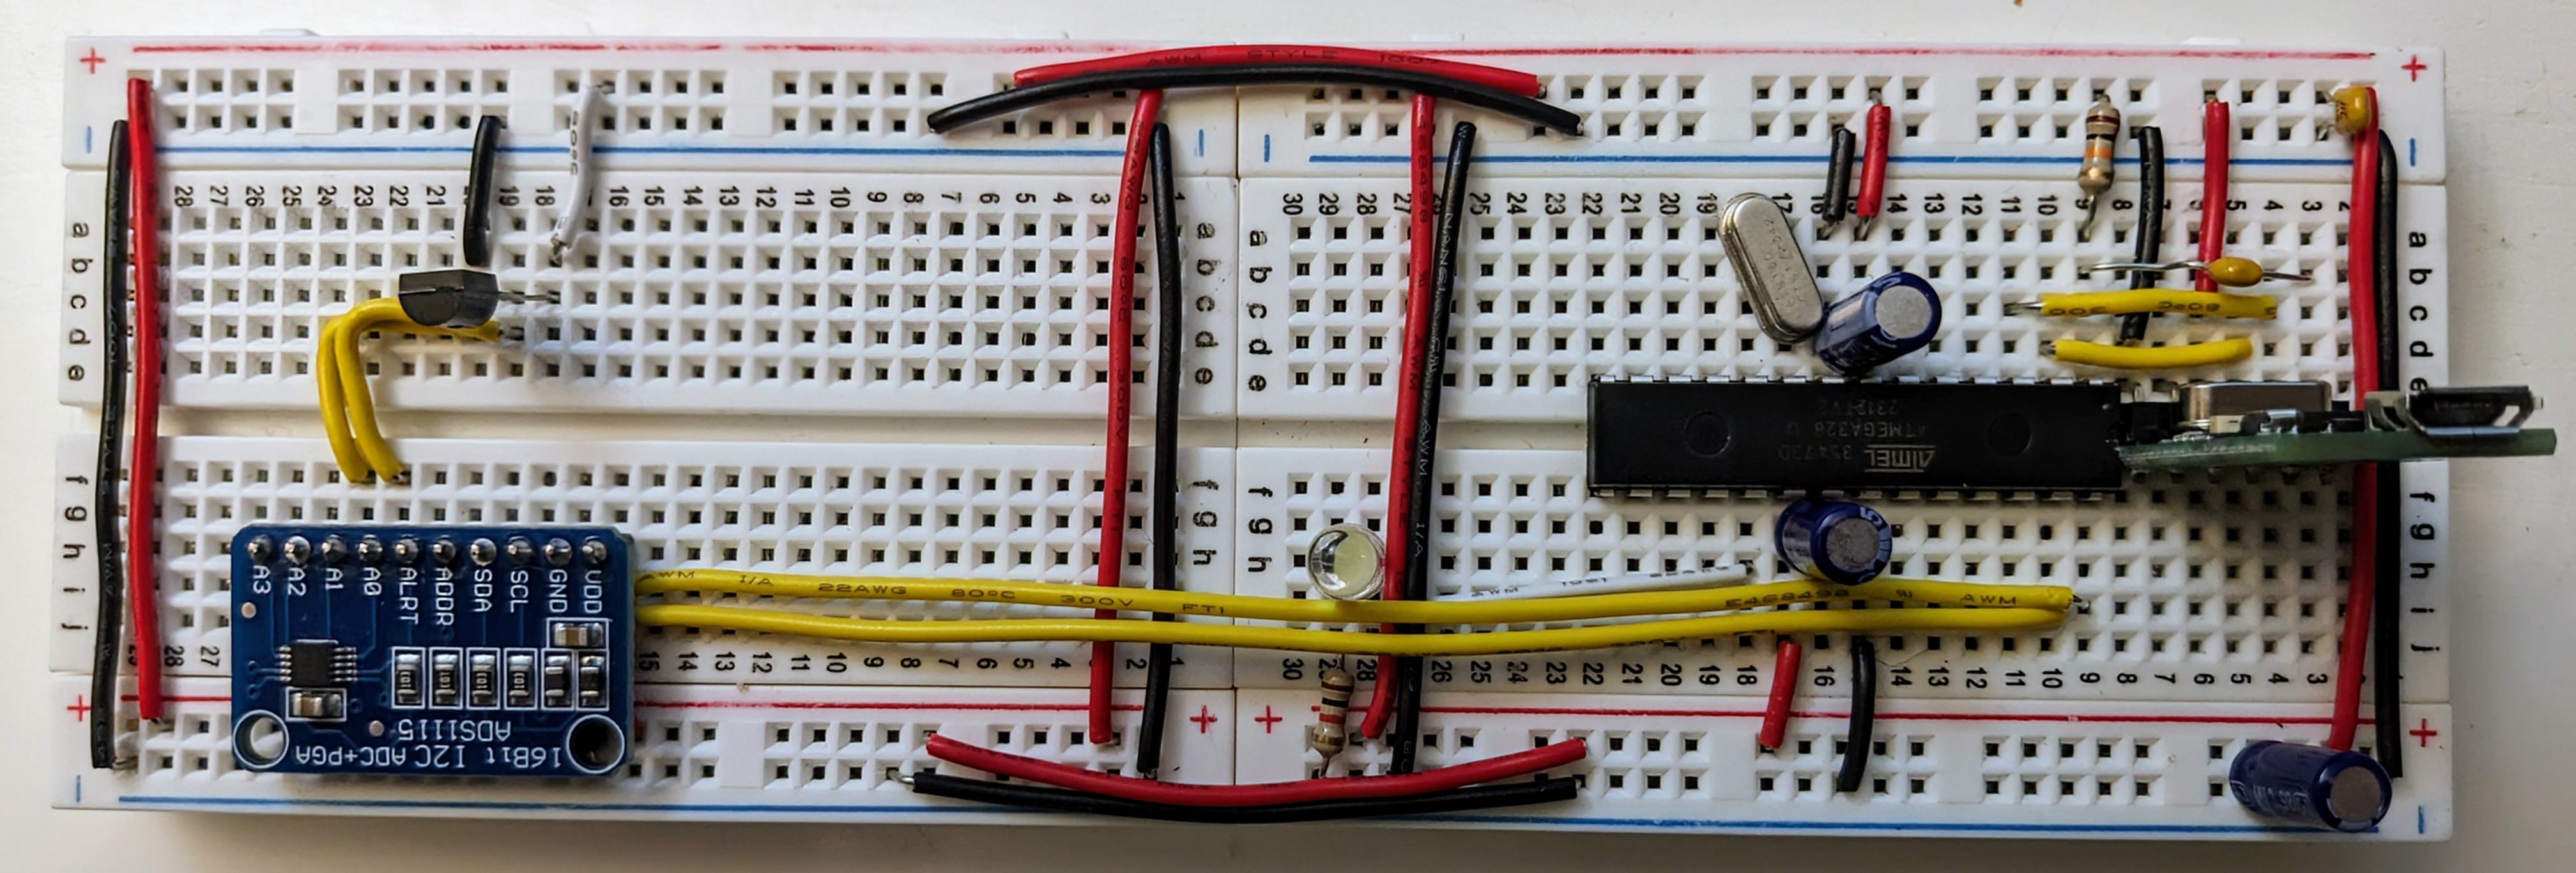
\includegraphics[scale=0.10]{figures/breadboard.jpg}
	\caption{Breadboard implementation}
\end{figure}

\begin{figure}[H]
	\centering
	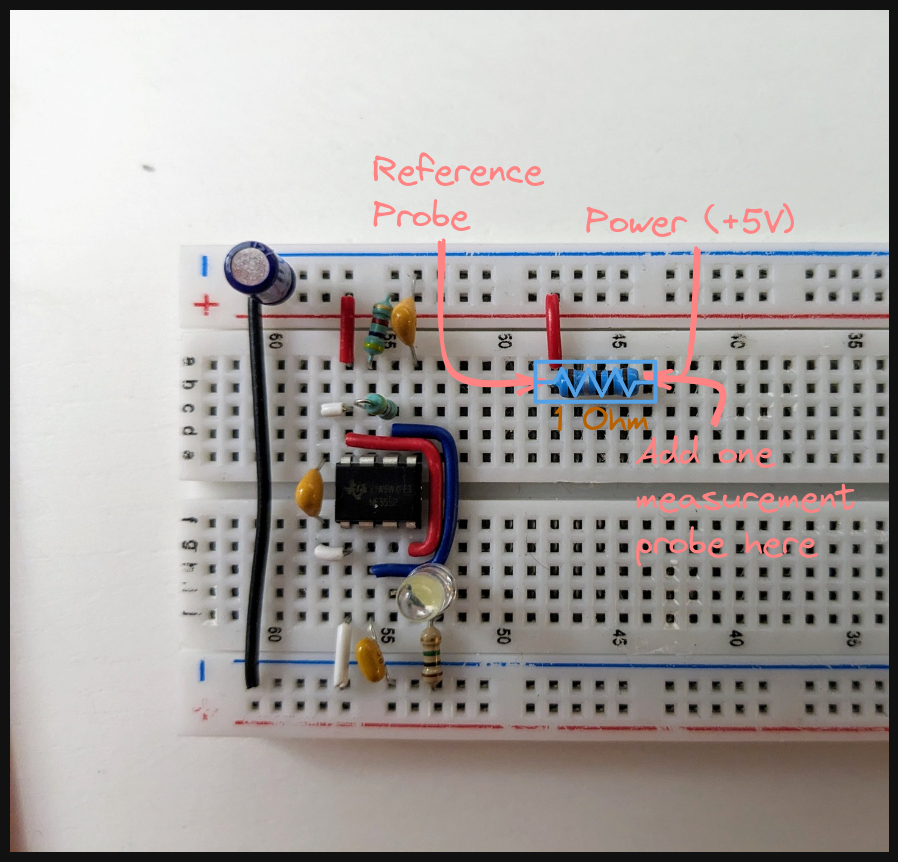
\includegraphics[scale=0.40]{figures/setup.png}
	\caption{Setup}
\end{figure}

\begin{figure}[H]
	\centering
	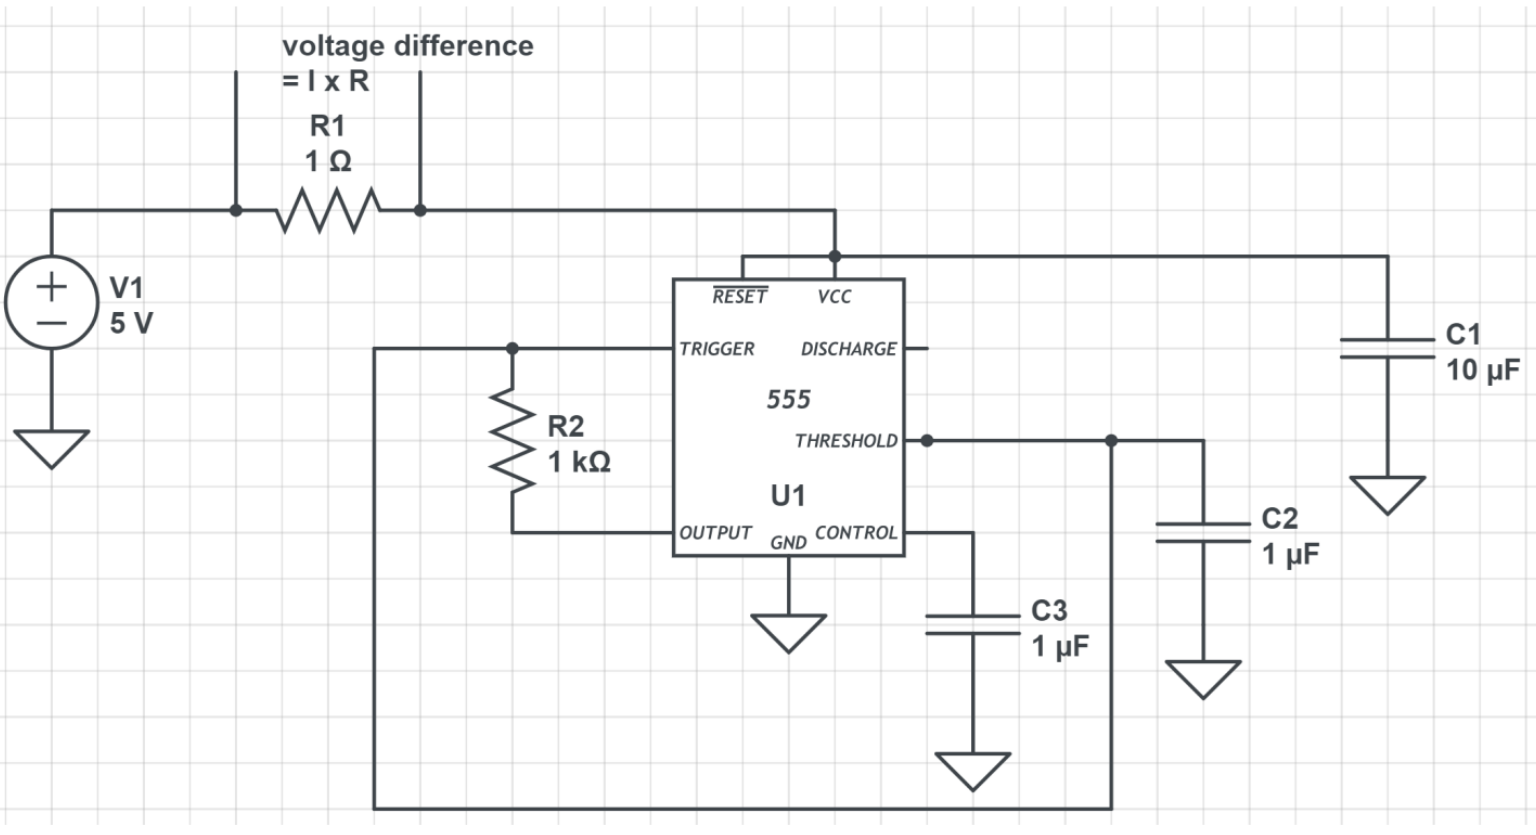
\includegraphics[scale=0.30]{figures/block_diagram.png}
	\caption{Block Diagram}
\end{figure}


\section{Component listing}


\begin{table}[!h]
	\centering

	\begin{tabular}{l c c c}
		\hline
		\textbf{Component Name} & \textbf{Usecase}               & \textbf{Symbol} & \textbf{Value} \\\hline
		                        &                                &                                  \\
		1 x Capacitor           & Charging Discharging Capacitor & C5              & 1$\mu$F        \\
		1 x Capacitor           & Decoupling cap                 & C5              & 22$\mu$F       \\
		1 x Capacitor           & Filter Capacitor               & C5              & 10$\mu$F       \\
		2 x Resistor            & Discharging rate Resistor      & R3              & 1k$\ohm$       \\
		1 x Resistor            & Inrush measurement Resistor    & R4              & 1$\ohm$        \\
		1 x Resistor            & Current Limiting resistor      & R5              & 1k$\ohm$       \\
		1x NE555                & Timer IC                       & U1                               \\
		1 x LEDs                & For output                     & LED                              \\
		\hline\hline
	\end{tabular}
	\caption{Components}
\end{table}





\section{Explanation}

\begin{itemize}
	\item \textbf{Series Sense Resistor:} the current measurement method used in this lab is the introduction of a series sense resistor in the power supply path. The sense resistor acts as a current-to-voltage converter, using the fundamental principle of Ohm's law, which states that the voltage across a resistor is directly proportional to the current flowing through it. By selecting an appropriate value for the sense resistor, a measurable voltage drop can be obtained without significantly affecting the circuit's power supply voltage.
\end{itemize}

The selection of the sense resistor value is a critical aspect of the measurement setup. The resistor value should be chosen to provide a voltage drop that is large enough to be accurately measured by the oscilloscope while minimizing the impact on the circuit's performance. A lower resistance value will result in a smaller voltage drop, reducing the measurement resolution and potentially introducing noise. Conversely, a higher resistance value will produce a larger voltage drop but may cause an excessive voltage drop in the power rail, affecting the circuit's operation. Therefore, a balance must be struck between measurement sensitivity and circuit functionality.

\begin{itemize}
	\item \textbf{Inrush Current:} Inrush current refers to the sudden and substantial current drawn by a circuit when power is initially applied. This current surge is primarily caused by the charging of capacitive elements within the circuit, such as decoupling capacitors. Decoupling capacitors are placed near integrated circuits and other components to provide a stable and locally filtered power supply, reducing noise and voltage fluctuations.\\
	      At the instant of power-on, the decoupling capacitors act as short circuits, allowing a large current to flow as they charge up to the power supply voltage. The magnitude and duration of the inrush current depend on several factors, including the power supply's characteristics (e.g., voltage, current limiting), the total capacitance of the decoupling capacitors, and the resistance of the current path.
\end{itemize}


Measuring the inrush current helps determine the maximum current handling capability required for the power supply and circuit components. If the inrush current exceeds the rated limits, it can potentially damage components or cause voltage drops that disrupt the circuit's operation. Secondly, understanding the inrush current characteristics enables to select appropriate protection mechanisms, such as soft-start circuits or inrush current limiters, to mitigate the effects of the current surge.

\begin{itemize}
	\item \textbf{Steady-State Current:} The steady-state current represents the current consumed by the circuit during normal operation, after the initial transients have settled. This current is determined by the active components, such as integrated circuits, transistors, and other devices, as well as the passive elements like resistors and LEDs.
\end{itemize}


\textbf{Oscilloscope Measurement:} Measuring the voltage across the sense resistor requires the use of an oscilloscope with two single-ended probes. The probes are connected to either side of the sense resistor, with both probes referenced to the circuit's local ground. This configuration allows for the measurement of the differential voltage across the resistor, eliminating the need for a differential probe or a ground-referenced measurement. The oscilloscope's triggering is set to the rising edge of the voltage across the sense resistor for inrush current measurement.

To obtain the current values from the voltage measurements, Ohm's law is applied. The measured voltage drop across the sense resistor is divided by the resistor value to calculate the corresponding current. This calculation is performed for both the steady-state and inrush current measurements.
\begin{itemize}
	\item \textbf{Decoupling Capacitor Variation:} The impact of decoupling capacitors on the inrush current can be investigated by varying the capacitor values in the circuit.
	\item By changing the decoupling capacitor values and measuring the resulting inrush current, the relationship between capacitance and inrush current can be analyzed. Larger capacitance values results in higher inrush currents and longer settling times, as more charge is required to reach the steady-state voltage. Conversely, smaller capacitance values lead to lower inrush currents and faster settling times.
\end{itemize}




\textbf{Limitations and Considerations:} While the current measurement technique using a series sense resistor is straightforward, there are certain limitations and considerations to keep in mind. The introduction of the sense resistor adds a small amount of resistance to the power supply path, which can affect the circuit's performance, particularly in low-voltage or high-current applications. The resistor's power rating must also be considered to ensure it can handle the expected current levels without overheating or failing.


\section{Procedure}
\begin{enumerate}
	\item Circuit Design and Construction:
	      \begin{itemize}
		      \item A simple 555 timer circuit was chosen as the test case.
		      \item Design the 555 timer circuit to generate a square wave output with a 50\% duty cycle. The circuit should include a decoupling capacitor on the power rail and an LED connected to the output through a current-limiting resistor.
		      \item Calculate the expected steady-state current based on the circuit parameters.
		      \item Construct the 555 timer circuit on a breadboard, incorporating the series sense resistor between the power supply and the circuit.
	      \end{itemize}
	\item Oscilloscope Setup:
	      \begin{itemize}
		      \item Connect two single-ended oscilloscope probes to the circuit. Place one probe on the high side of the sense resistor and the other probe on the low side of the resistor. Ensure both probes are referenced to the circuit's local ground.
		      \item Set the oscilloscope to measure the voltage difference between the two probes. This can be achieved using the oscilloscope's built-in math functions or by manually subtracting the voltages.
		      \item Adjust the oscilloscope's vertical scale settings to accurately capture the small voltage drop across the sense resistor. A vertical scale of 10 mV/div or lower.
		      \item Set the oscilloscope's triggering to capture the relevant waveforms. For steady-state current measurement, trigger on the 555 timer's output signal. For inrush current measurement, trigger on the rising edge of the voltage across the sense resistor.
	      \end{itemize}
	\item Steady-State Current Measurement:
	      \begin{itemize}
		      \item Power on the 555 timer circuit and allow it to reach steady-state operation.
		      \item Observe the voltage waveform across the sense resistor on the oscilloscope. Measure the voltage drop when the LED is lit.
		      \item Calculate the steady-state current using Ohm's law, dividing the measured voltage drop by the sense resistor value.
		      \item  Compare the measured steady-state current with the expected value calculated in above step
	      \end{itemize}
	\item Inrush Current Measurement:
	      \begin{itemize}
		      \item Set the oscilloscope to trigger on the rising edge of the voltage across the sense resistor. Adjust the trigger level to capture the inrush current waveform accurately.
		      \item Disconnect and reconnect the power supply to the 555 timer circuit while monitoring the oscilloscope display.
		      \item Capture the inrush current waveform on the oscilloscope. Measure the peak voltage drop across the sense resistor during the inrush event. with math function by subtracting both differential ends of oscilloscope probes
		      \item Calculate the peak inrush current using Ohm's law, dividing the measured peak voltage drop by the sense resistor value.
		      \item Observe the duration of the inrush current and note any relevant characteristics, such as the time taken for the current to settle to the steady-state value.
	      \end{itemize}
	\item Decoupling Capacitor Variation:
	      \begin{itemize}
		      \item Modify the value of the decoupling capacitor in the 555 timer circuit to investigate its impact on the inrush current.
		      \item Repeat steps for decoupling capacitor value tested.
		      \item Compare the inrush current waveforms and peak values obtained for different decoupling capacitor values.
		      \item Analyze the relationship between the decoupling capacitor value and the inrush current characteristics.
	      \end{itemize}
\end{enumerate}

\section{Measurement}
\begin{enumerate}
	\item Steady-State Current Measurement:
	      \begin{itemize}
		      \item Oscilloscope Settings: \\
		            - Channel 1: Connected to the high side of the sense resistor \\
		            - Channel 2: Connected to the low side of the sense resistor \\
		            - Math Function: Ch1 - Ch2 (to calculate the voltage difference across the sense resistor) \\
		            - Vertical Scale: 100 mV/div \\
		            - Horizontal Scale: 5 ms/div \\
		            - Trigger: Channel 1, rising edge, trigger level set to capture the steady-state waveform \\
		      \item Measurement Procedure: \\
		            - Power on the 555 timer circuit and allow it to reach steady-state operation. \\
		            - Observe the voltage waveform across the sense resistor on the oscilloscope. \\
		            - Measure the voltage drop ( $\Delta$ V) across the sense resistor when the LED is lit. \\
		            - Calculate the steady-state current (I) using Ohm's law: I = $\frac{\Delta V}{R}$ , where R is the sense resistor value.
		      \item Results: \\
		            - Sense Resistor Value (R): 1 $\ohm$ \\
		            - Measured Voltage Drop (delta V): 1.4 mV \\
		            - Calculated Steady-State Current (I):I = $\frac{1.4mV}{1 \ohm}$ = 1.4 mA
		      \item \textbf{The measured steady-state current of 1.4 mA, now practically we have seen voltage drop of 1V across output of 555 so we can calculate theoretical value for current which would be,\\
			            I\_theoretical = $\frac{1mV}{1 k\ohm}$ = 1 mA, which closely matches the result}

		            \begin{figure}[H]
			            \centering
			            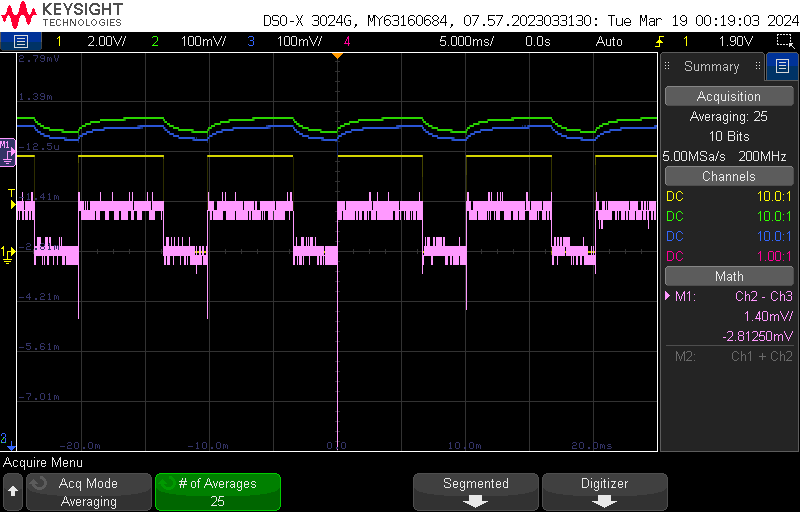
\includegraphics[scale=0.6]{figures/steady_state1.png}
			            \caption{Steady state current}
		            \end{figure}
	      \end{itemize}
	\item Inrush Current Measurement:
	      \begin{itemize}
		      \item Oscilloscope Settings: \\
		            - Channel 1: Connected to the high side of the sense resistor\\
		            - Channel 2: Connected to the low side of the sense resistor\\
		            - Math Function: Ch1 - Ch2 (to calculate the voltage difference across the sense resistor)\\
		            - Vertical Scale: 2 V/div (adjust as needed to capture the inrush current peak) \\
		            - Horizontal Scale: 5 us/div  \\
		            - Trigger: Channel 1, rising edge, trigger level set to capture the inrush current waveform\\
		      \item Measurement Procedure:\\
		            - Set the oscilloscope to trigger on the rising edge of the voltage across the sense resistor. \\
		            - Disconnect and reconnect the power supply to the 555 timer circuit while monitoring the oscilloscope display. \\
		            - Capture the inrush current waveform on the oscilloscope. - Measure the peak voltage drop (delta V\_peak) across the sense resistor during the inrush event. \\
		            - Calculate the peak inrush current (I\_peak) using Ohm's law: I\_peak = delat V\_peak / R, where R is the sense resistor value.
		      \item Results: \\
		            - Sense Resistor Value (R): 1 ohm - Measured Peak Voltage Drop (delta V\_peak): 1.3 V \\
		            - Calculated Peak Inrush Current (I\_peak): I\_peak = 1.3 V / 1 ohm = 1.3 A \\
		            - Inrush Current Duration: Approximately 20 us (time taken for the current to settle to the steady-state value)\\
		      \item \textbf{The peak inrush current of 1.3 A is significantly higher than the steady-state current, highlighting the importance of considering inrush current in circuit design and component selection.}

		            \begin{figure}[H]
			            \centering
			            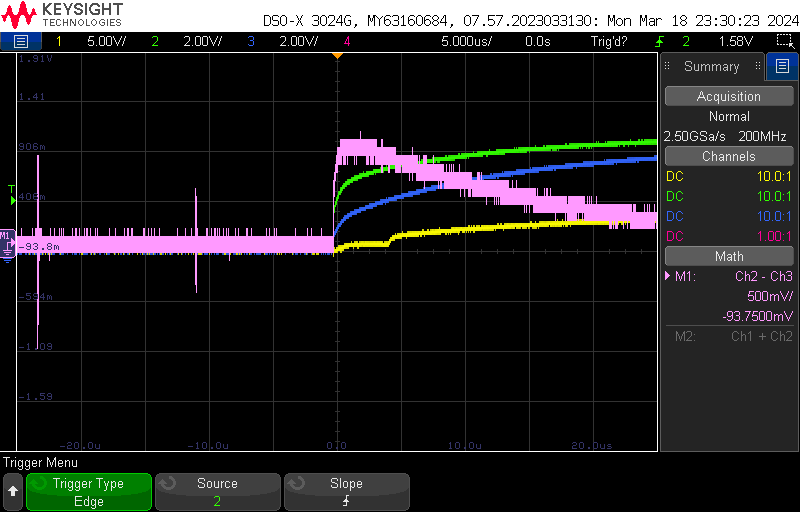
\includegraphics[scale=0.6]{figures/inrush_with_cap.png}
			            \caption{In rush current}
		            \end{figure}
	      \end{itemize}
	\item Decoupling Capacitor Variation:
	      \begin{itemize}
		      \item Measurement Procedure: \\
		            - Modify the value of the decoupling capacitor in the 555 timer circuit.(remove capacitor) \\
		            - Repeat the inrush current measurement procedure without decoupling capacitor. \\
		            - Compare the inrush current waveforms and peak values obtained for different decoupling capacitor values.
		      \item Results:\\
		            - Decoupling Capacitor Values Tested: 0 µF(no decoupling capacitor)\\
		            - 0 µF:  Peak Inrush Current: 500mV / 1 ohm = 500mA Inrush Current Duration:  \textless5uS -

		            \begin{figure}[H]
			            \centering
			            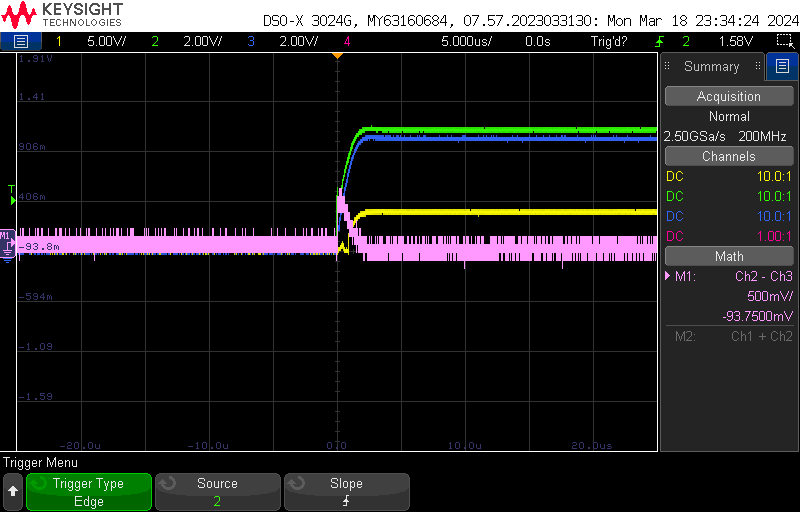
\includegraphics[scale=0.6]{figures/inrush_without_cap.png}
			            \caption{In rush current without decoupling capacitor}
		            \end{figure}
	      \end{itemize}
\end{enumerate}



\section{Learnings and Observation}
\begin{enumerate}
	\item \textbf{Understanding Inrush Current:} The lab demonstrated the significance of inrush current in electronic circuits. Inrush current refers to the sudden and substantial current drawn by a circuit when power is initially applied, primarily due to the charging of capacitive elements such as decoupling capacitors. The measurements showed that the inrush current can be significantly higher than the steady-state current, reaching values of 2 A in the tested circuit. This highlights the importance of considering inrush current in circuit design, component selection, and power supply sizing to ensure reliable operation and prevent damage to components.
	\item Steady-State Current Measurement:
	      \begin{itemize}
		      \item The steady-state current of the 555 timer circuit was successfully measured using a sense resistor and oscilloscope.
		      \item The measured steady-state current of 1.4 mA closely matches the theoretically calculated value of 1 mA, based on the observed voltage drop of 1 V across the output of the 555 timer and the 1 k$\ohm$ resistor.
		      \item This demonstrates the accuracy of the measurement technique and validates the theoretical understanding of the circuit's behavior.
	      \end{itemize}



	\item Inrush Current Measurement:\
	      \begin{itemize}
		      \item The inrush current of the 555 timer circuit was captured and measured using the oscilloscope.
		      \item The peak inrush current of 1.3 A is significantly higher than the steady-state current, highlighting the importance of considering inrush current in circuit design and component selection.
		      \item The inrush current duration of approximately 20 us indicates the time taken for the current to settle to the steady-state value.
		      \item This measurement provides valuable insights into the circuit's behavior during the initial power-on phase and emphasizes the need for proper inrush current management.
	      \end{itemize}
	\item Decoupling Capacitor Variation:\
	      \begin{itemize}
		      \item The impact of the decoupling capacitor on the inrush current characteristics was investigated by removing the capacitor from the 555 timer circuit.
		      \item Without the decoupling capacitor, the peak inrush current was measured to be 500 mA, which is lower than the peak inrush current with the capacitor in place.
		      \item The inrush current duration without the decoupling capacitor was less than 5 us, indicating a faster settling time compared to the case with the capacitor.
		      \item These results demonstrate the role of the decoupling capacitor in suppressing high-frequency noise and stabilizing the power supply, but also show its contribution to the inrush current.

	      \end{itemize}



\end{enumerate}

\section{Conclusion}

\begin{enumerate}
	\item The lab on measuring inrush current and steady-state current provided a comprehensive understanding of the power consumption characteristics of electronic circuits. Through practical measurements and analysis, the significance of inrush current, the impact of decoupling capacitors, and the importance of accurate current measurement techniques were demonstrated.

	\item The results obtained from the 555 timer circuit highlighted the substantial difference between inrush current and steady-state current, emphasizing the need to consider inrush current in circuit design and component selection. The peak inrush current of 1.3 A observed in the circuit underscores the potential for component stress and the necessity of appropriate protection mechanisms.

	\item The steady-state current measurement of 1.4 mA closely matched the expected value, validating the LED current estimation and providing insights into the circuit's power consumption during normal operation.

	\item The investigation of decoupling capacitor variation revealed the relationship between capacitance and inrush current characteristics. Larger capacitance values resulted in higher peak inrush currents and longer settling times, highlighting the trade-offs involved in selecting decoupling capacitors for noise reduction and inrush current management.
\end{enumerate}

\vspace{50px}
\hrule
\hrule

\pagebreak





%---------------------------------------------------------------------------
\end{document}

